\subsection{Simulation }
Our simulation is based on two softwares: MATLAB(SimBiology Toolbox) and COPASI.

SimBiology Toolbox provides functions for modeling, simulating, and analyzing biochemical pathways by the powerful computing engine of MATLAB.

\begin{figure}[h]
	\centering
	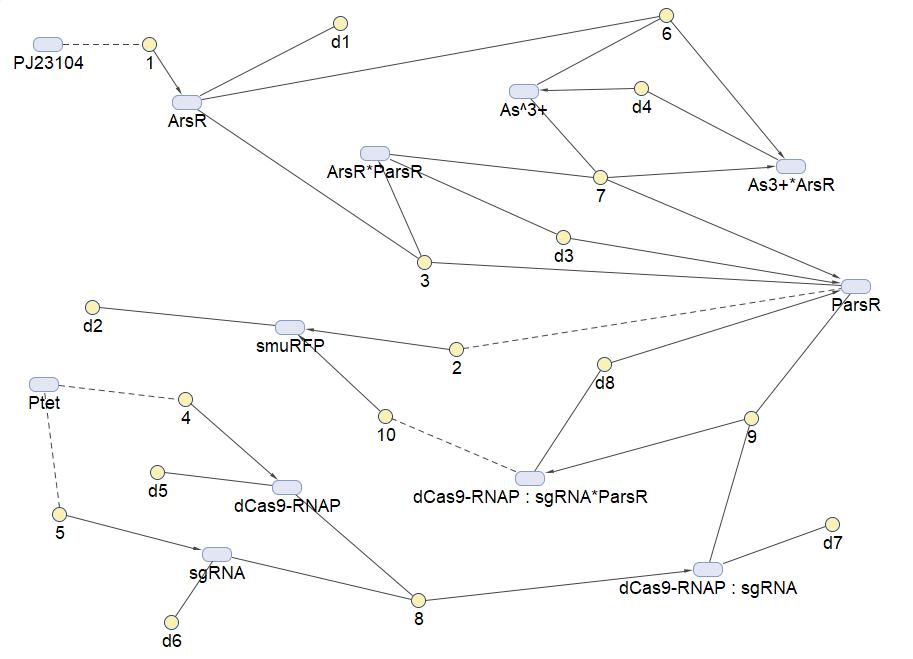
\includegraphics[width=10cm]{screenshot003}	
	\caption{Reaction map generated from the reaction sets above by SimBiology Toolbox}
\end{figure}



\begin{figure}[H]
	\centering
	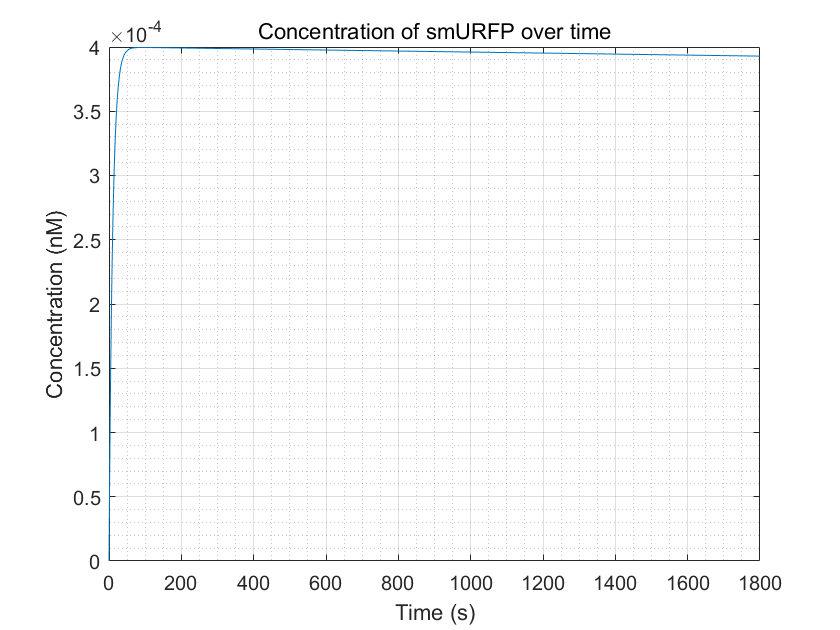
\includegraphics[width=10cm]{11}
	\caption{Simulation of smURFP production as a function of time by MATLAB}
\end{figure}

Through the figure, we can see that the smURFP can gradually increase and reach a steady state after a period in the presence of arsenic ions.

\subsection{Sensitivity }
A good biosystem should have certain stability towards fluctuations in parameters. A good model should reflect this, and hence a test for robustness can be essential to the model.

Robustness analysis can also pinpoint which reactions/parameters that are important for obtaining a specific biological behavior. A simple measure for sensitivity is to measure the relative change of a system feature due to a change in a parameter. As for our model, the feature can be the equilibrium concentration of the smURFP(C) for which the sensitivity (S) to a parameter k is:
\begin{equation}
	S=\frac{\frac{dC}{C}}{\frac{dk}{k}}=\frac{dC}{dk}\frac{k}{c}\approx \frac{\Delta C}{\Delta k}\frac{k}{c}
\end{equation}
After analysis, we found that the concentration of smURFP is relatively sensitive to parameters such as ktx3, ktl3, ktx4, kb4, kb6, kd2, kd5, kd6, kd7, kd8, kd11, etc. Among these parameters, except for the parameters that directly affect the formation and degradation of smURFP, the rest of them are all related to dCas9-RNAP and sgRNA. This shows that our model reflects  important role of dCas9 , which initially confirms our hypothesis: dCas9-RNAP can enhance transcription to increase the concentration of SmURFP. However, due to the lack of previous modeling studies on dCas9-RNAP, some kinetic parameters are not very accurate, and due to experimental conditions, we can not design experiments to measure related parameters, which led to some deviations in our model -- The concentration of fluorescent egg smURFP is not high enough, so we have put forward a bold hypothesis to speculate on how much fluorescence intensity can be theoretically increased by the introduction of dCas9-RNAP.\\
The sensitivity of each parameter is shown in the figures below.
\begin{figure}[H]
	\centering
	\begin{subfigure}{0.5\textwidth}
		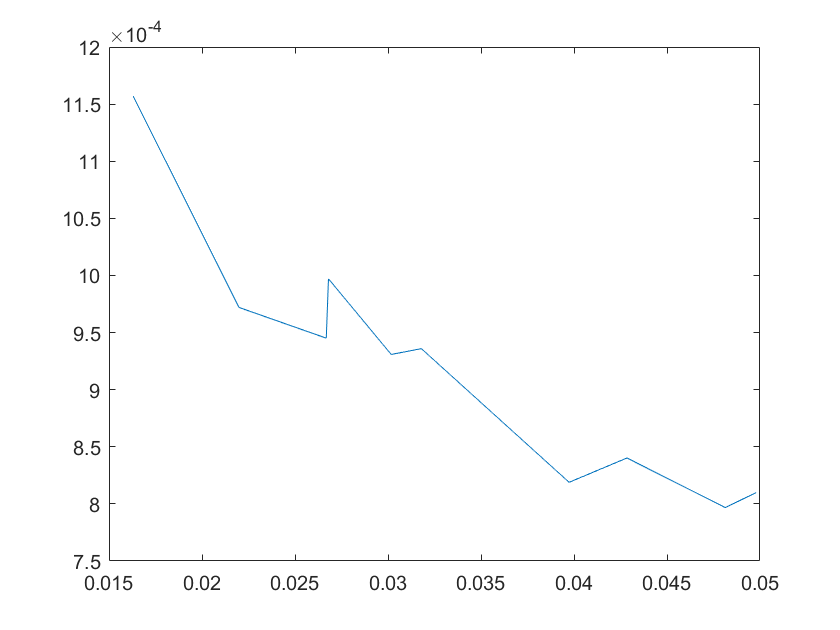
\includegraphics[height=4cm]{tx1.png}
		\caption{sensitivity of ktx1}
	\end{subfigure}
	\begin{subfigure}{0.5\textwidth}
		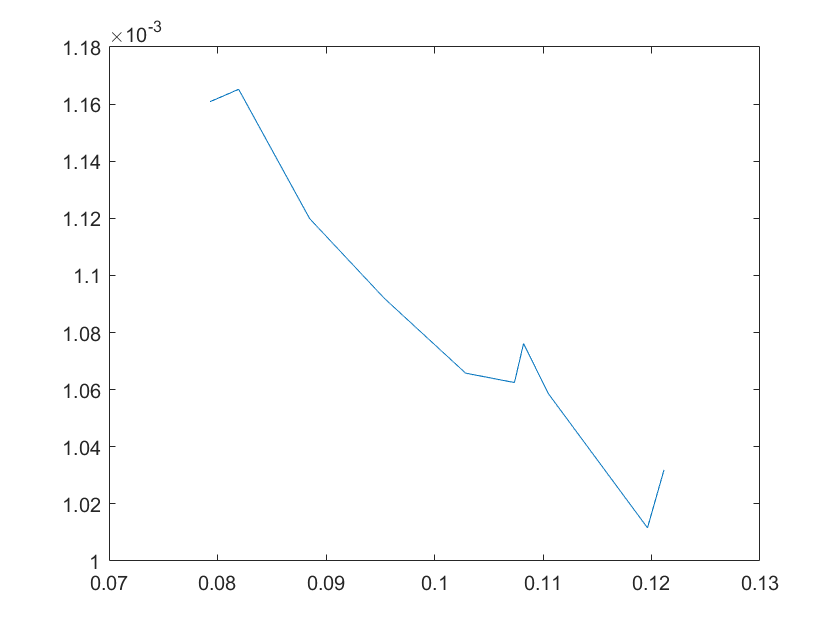
\includegraphics[height=4cm]{tl1.png}
		\caption{sensitivity of ktl1}
	\end{subfigure}
	\begin{subfigure}{0.5\textwidth}
		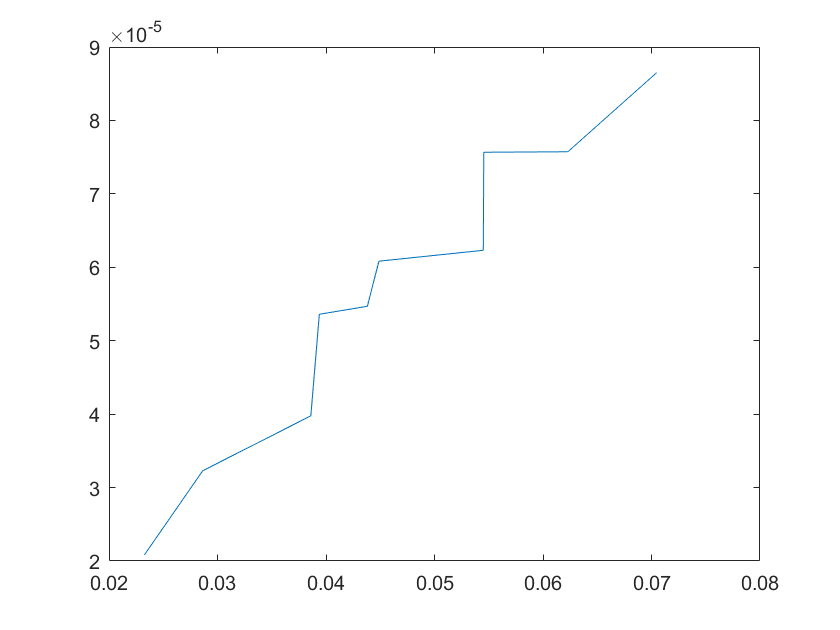
\includegraphics[height=4cm]{tx2.png}
		\caption{sensitivity of ktx2}
	\end{subfigure}%
	\begin{subfigure}{0.5\textwidth}
		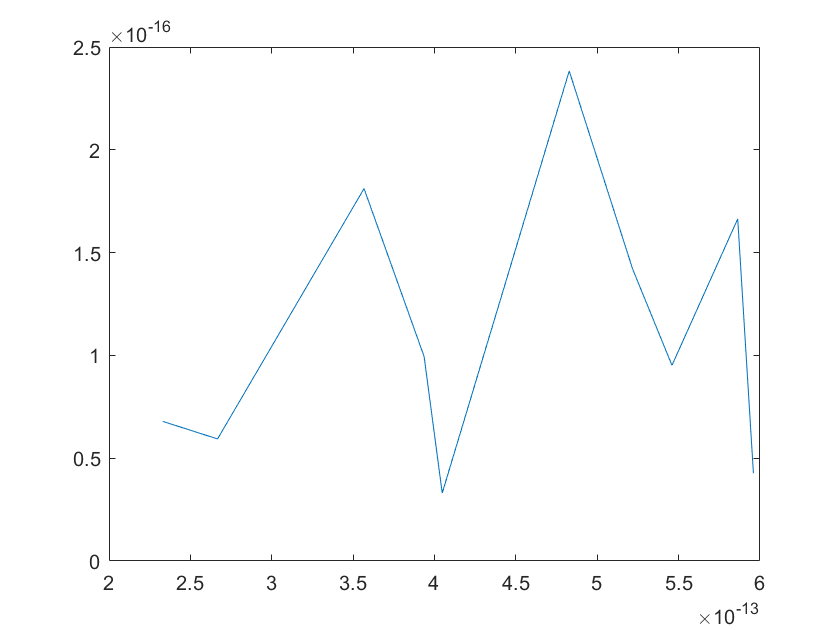
\includegraphics[height=4cm]{tl2.png}
		\caption{sensitivity of ktl2}
	\end{subfigure}
	\begin{subfigure}{0.5\textwidth}
		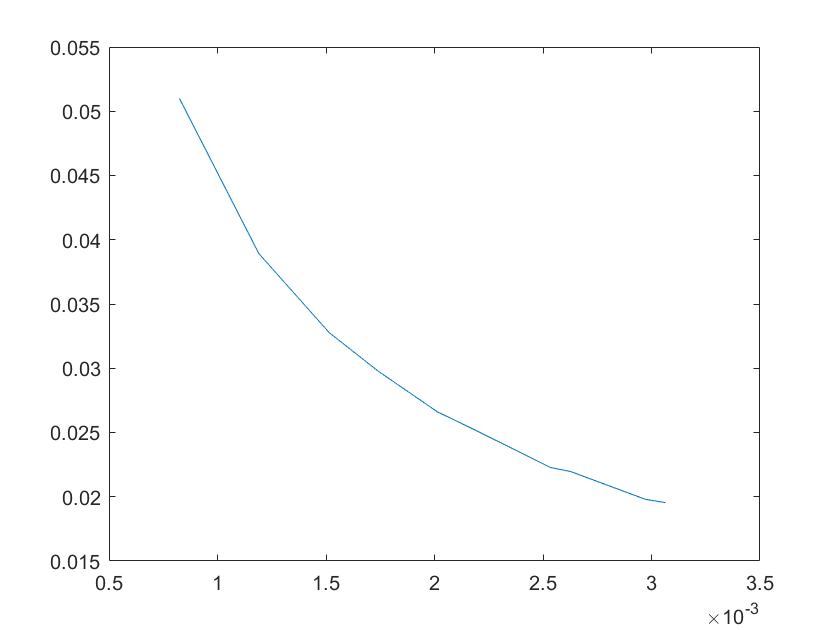
\includegraphics[height=4cm]{tx3.png}
		\caption{sensitivity of ktx3}
	\end{subfigure}%
	\begin{subfigure}{0.5\textwidth}
		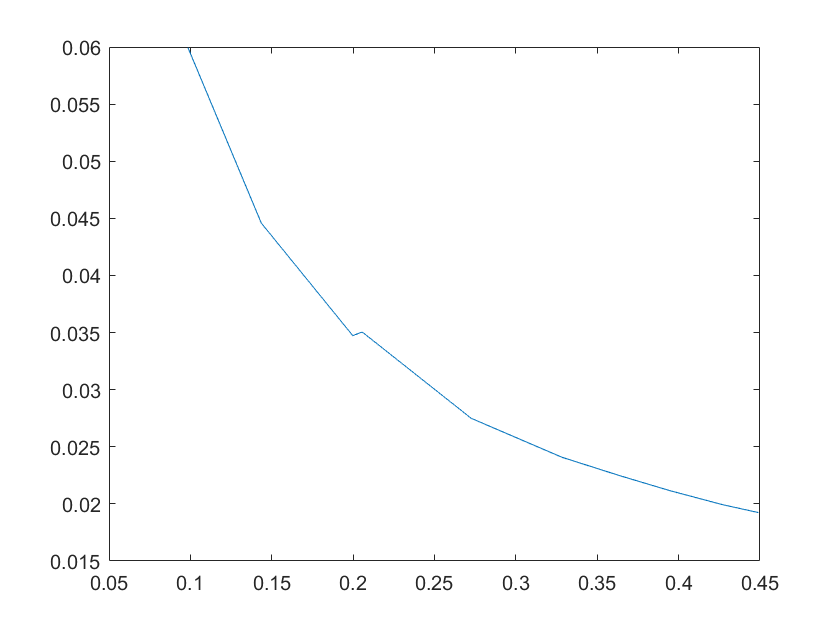
\includegraphics[height=4cm]{tl3.png}
		\caption{sensitivity of ktl3}
	\end{subfigure}
	\begin{subfigure}{0.5\textwidth}
		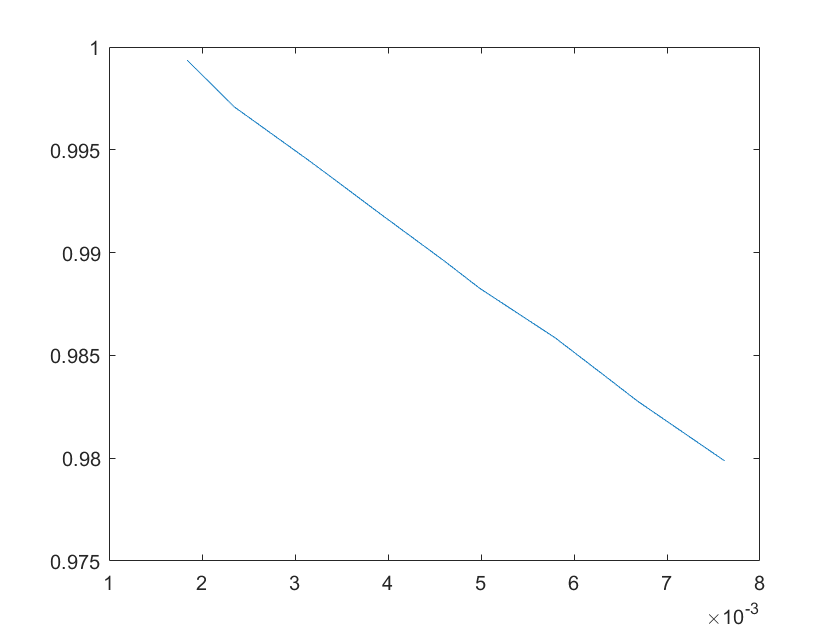
\includegraphics[height=4cm]{tx4.png}
		\caption{sensitivity of ktx4}
	\end{subfigure}%
	\begin{subfigure}{0.5\textwidth}
		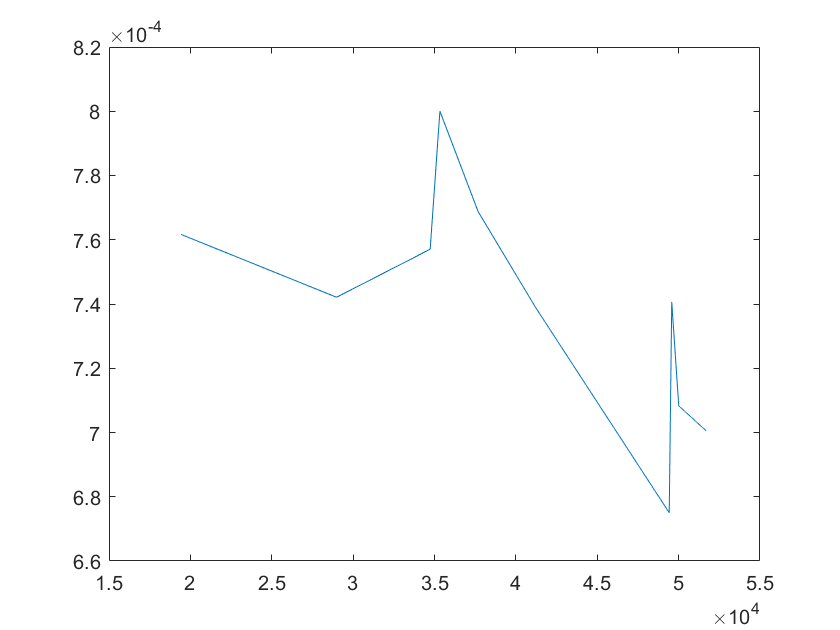
\includegraphics[height=4cm]{b1.png}
		\caption{sensitivity of kb1}
	\end{subfigure}
	\begin{subfigure}{0.5\textwidth}
		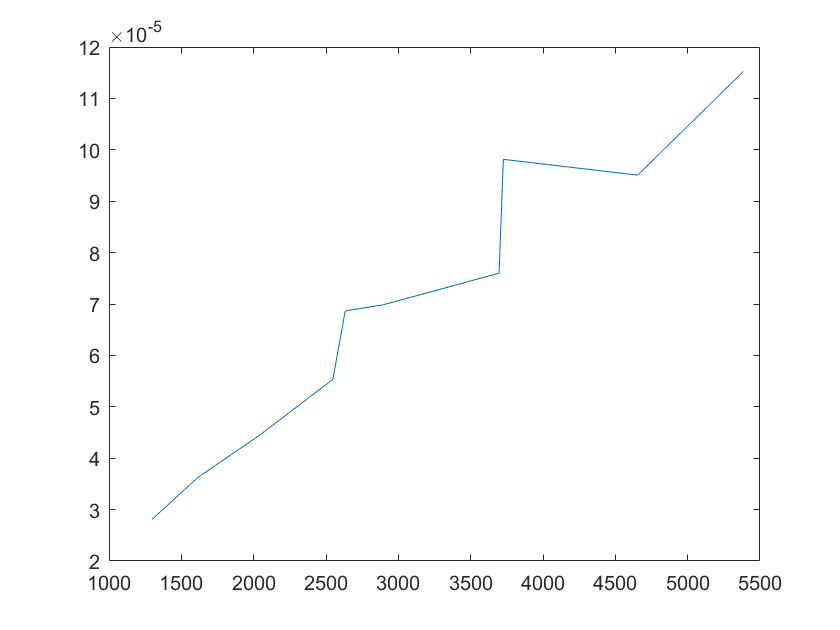
\includegraphics[height=4cm]{b2.png}
		\caption{sensitivity of kb2}
	\end{subfigure}%
	\begin{subfigure}{0.5\textwidth}
		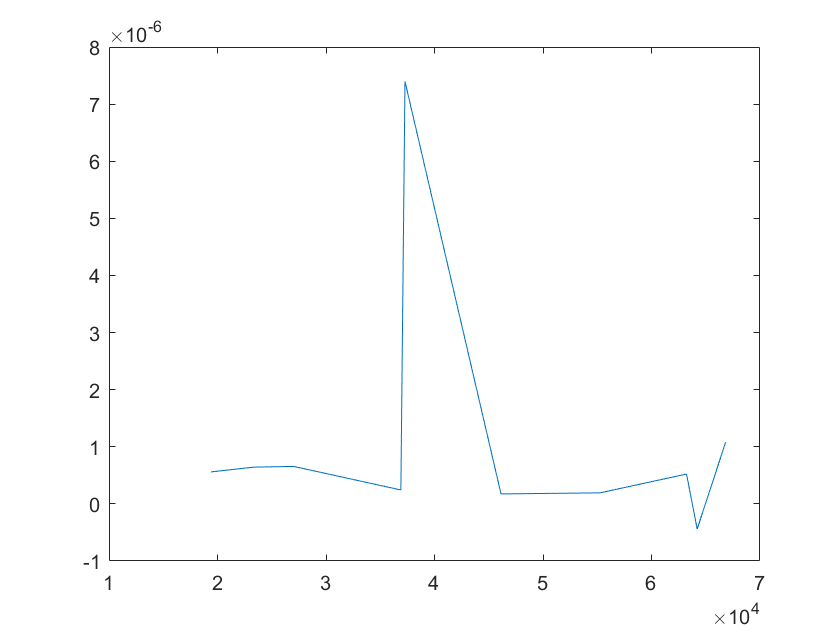
\includegraphics[height=4cm]{b3.png}
		\caption{sensitivity of kb3}
	\end{subfigure}
	\caption{Sensitivity analysis of ktx1-kb3}
\end{figure}

\begin{figure}[H]
	\begin{subfigure}{0.5\textwidth}
		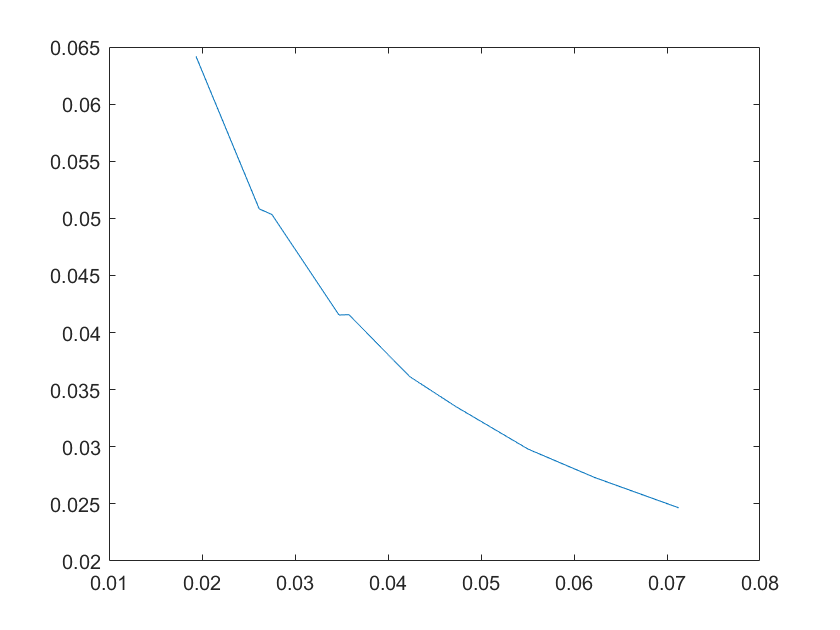
\includegraphics[height=4cm]{b4.png}
		\caption{sensitivity of kb4}
	\end{subfigure}%
	\begin{subfigure}{0.5\textwidth}
		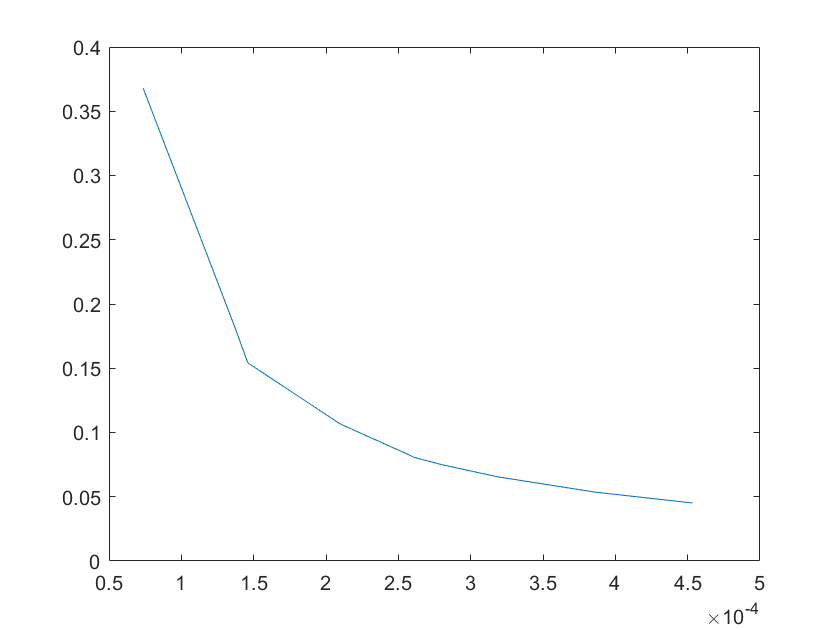
\includegraphics[height=4cm]{b5.png}
		\caption{sensitivity of kb5}
	\end{subfigure}
	\begin{subfigure}{0.5\textwidth}
		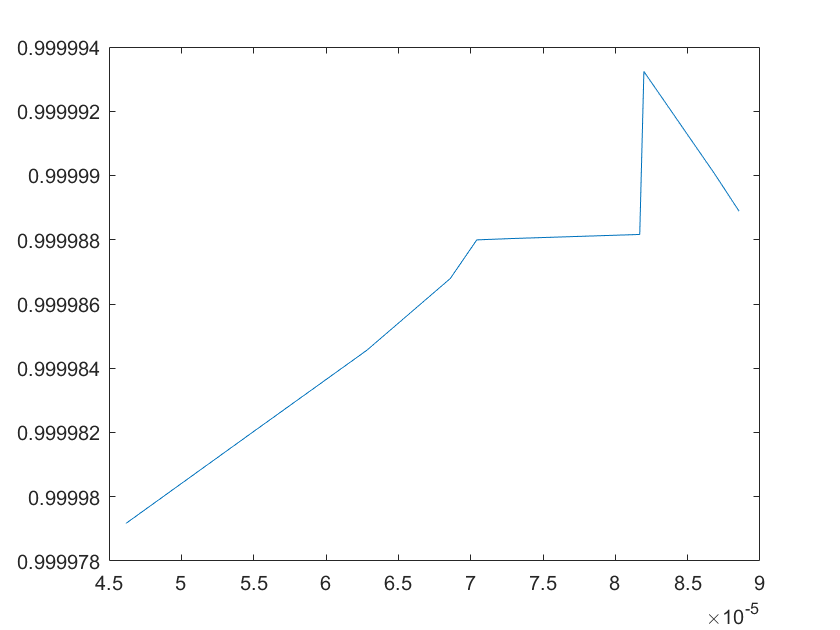
\includegraphics[height=4cm]{b6.png}
		\caption{sensitivity of kb6}
	\end{subfigure}%
	\begin{subfigure}{0.5\textwidth}
		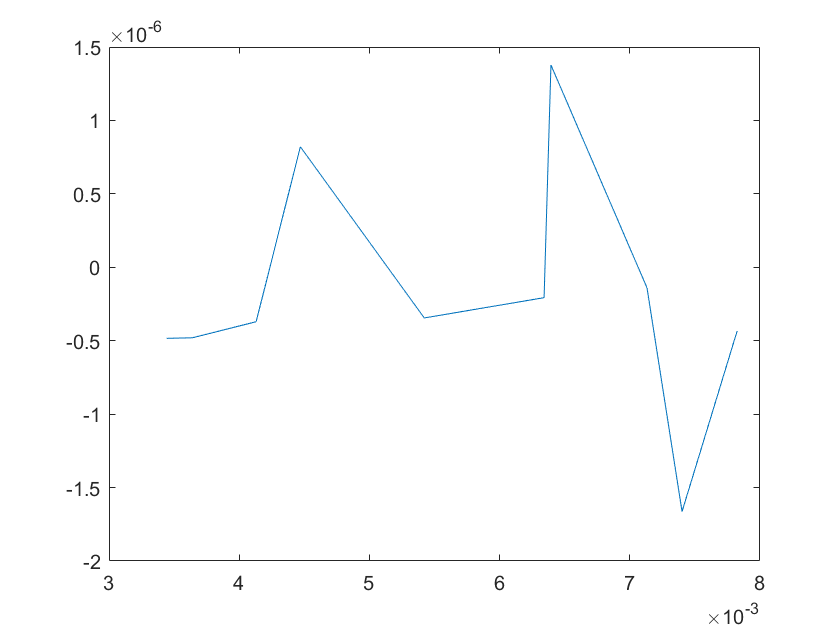
\includegraphics[height=4cm]{d1.png}
		\caption{sensitivity of kd1}
	\end{subfigure}
	\begin{subfigure}{0.5\textwidth}
		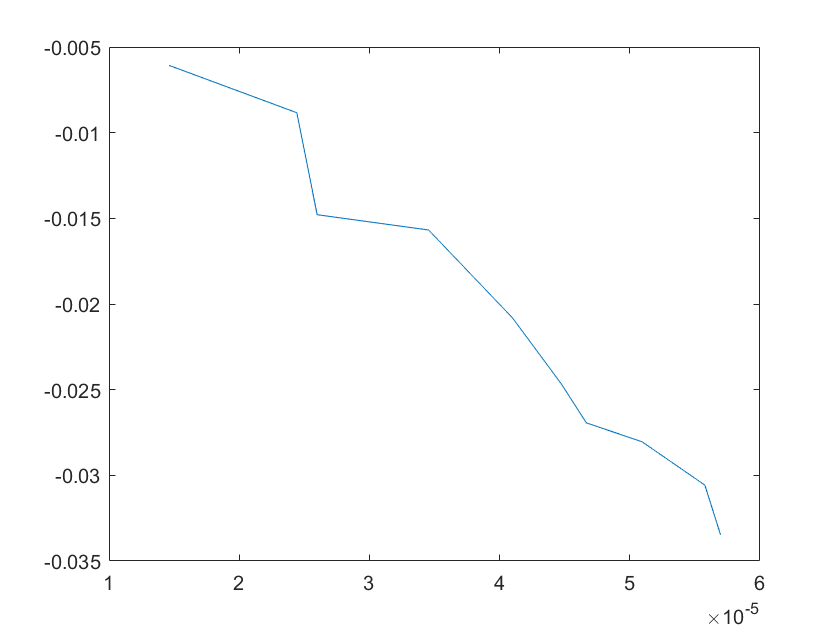
\includegraphics[height=4cm]{d2.png}
		\caption{sensitivity of kd2}
	\end{subfigure}%
	\begin{subfigure}{0.5\textwidth}
		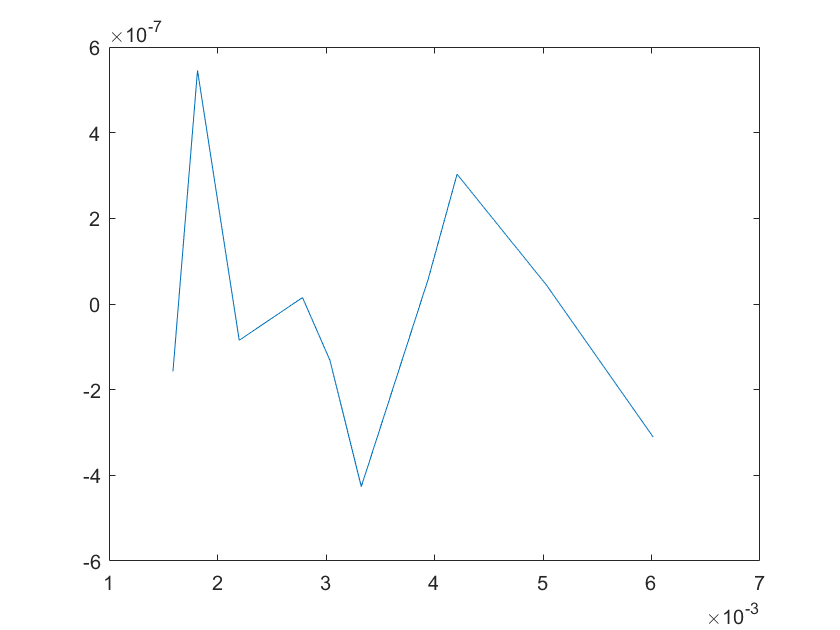
\includegraphics[height=4cm]{d3.png}
		\caption{sensitivity of kd3}
	\end{subfigure}
	\begin{subfigure}{0.5\textwidth}
		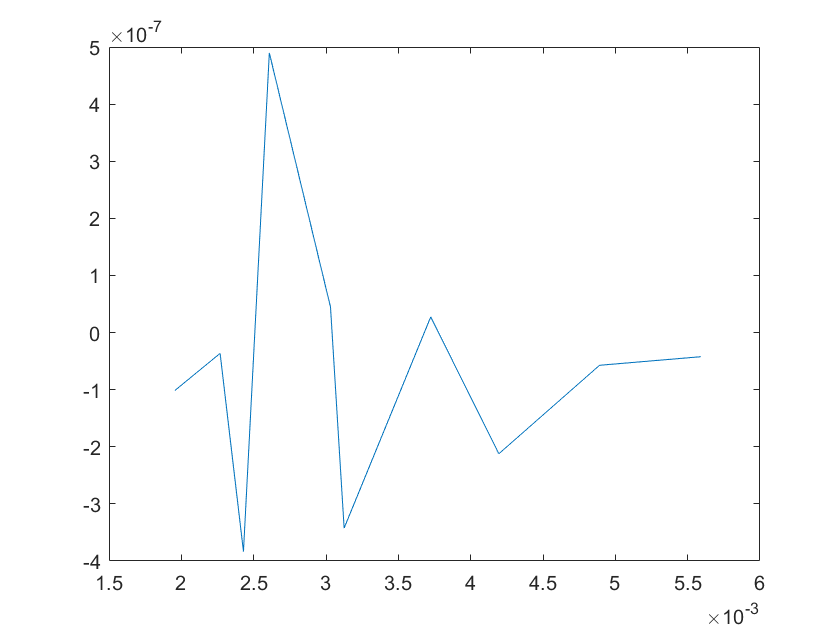
\includegraphics[height=4cm]{d4.png}
		\caption{sensitivity of kd4}
	\end{subfigure}%
	\begin{subfigure}{0.5\textwidth}
		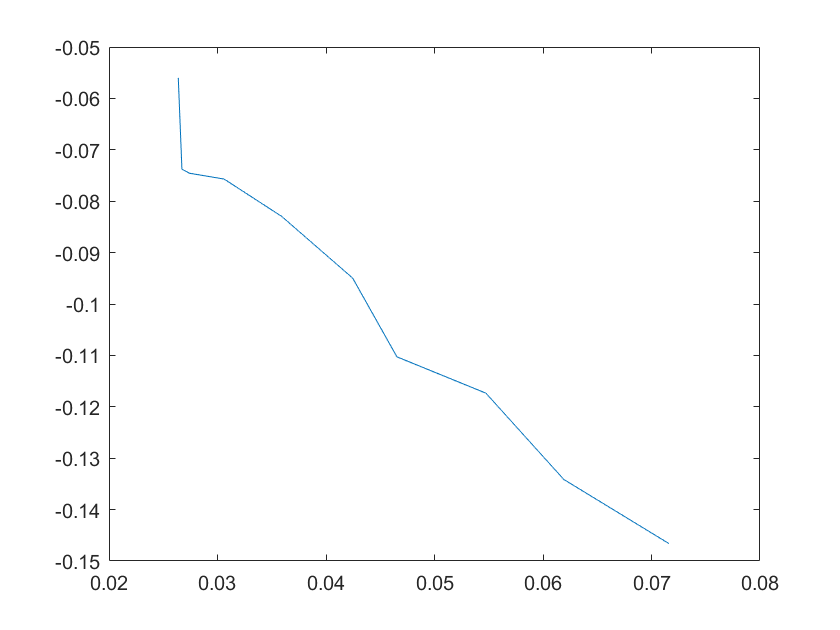
\includegraphics[height=4cm]{d5.png}
		\caption{sensitivity of kd5}
	\end{subfigure}
	\caption{Sensitivity analysis of kb4-kd5}
	
	\begin{figure}[H]
		\begin{subfigure}{0.5\textwidth}
			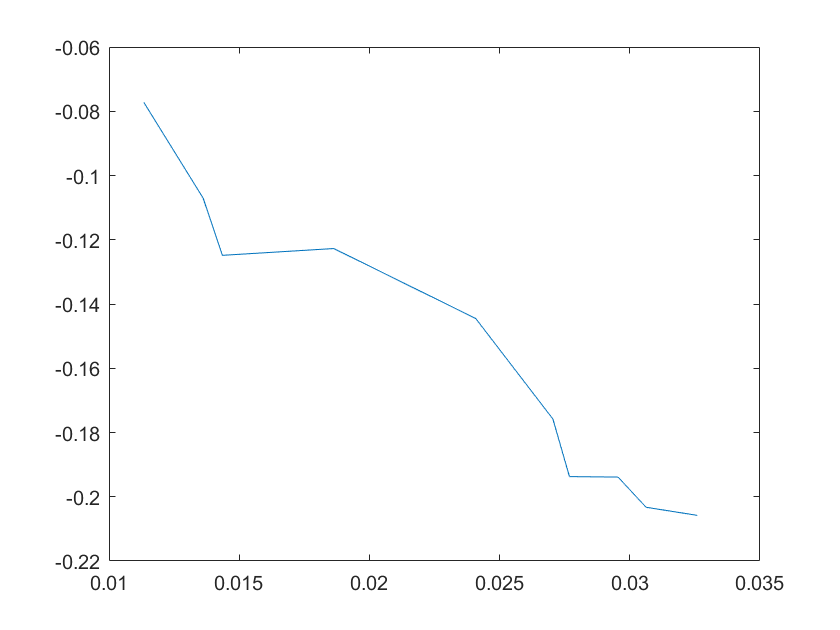
\includegraphics[height=4cm]{d6.png}
			\caption{sensitivity of kd6}
		\end{subfigure}%
		\begin{subfigure}{0.5\textwidth}
			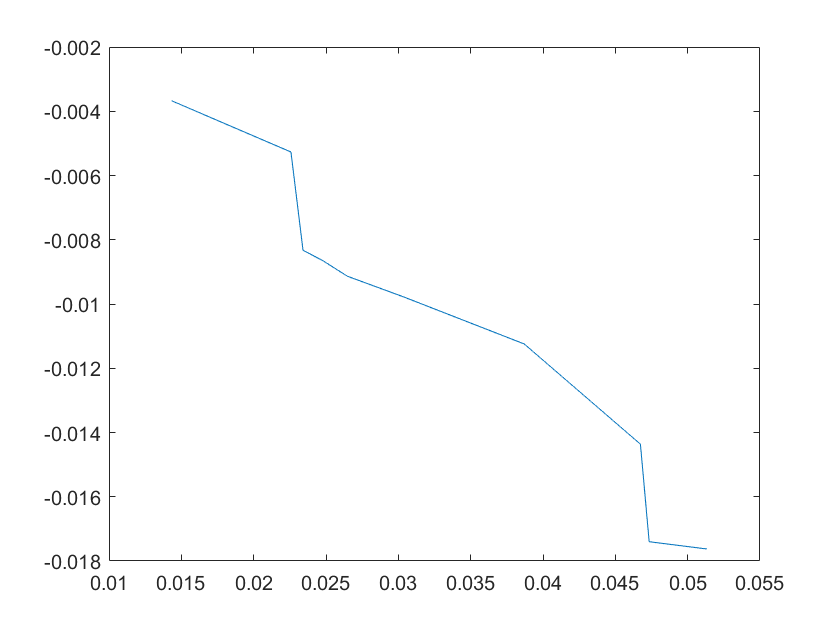
\includegraphics[height=4cm]{d7.png}
			\caption{sensitivity of kd7}
		\end{subfigure}
		\begin{subfigure}{0.5\textwidth}
			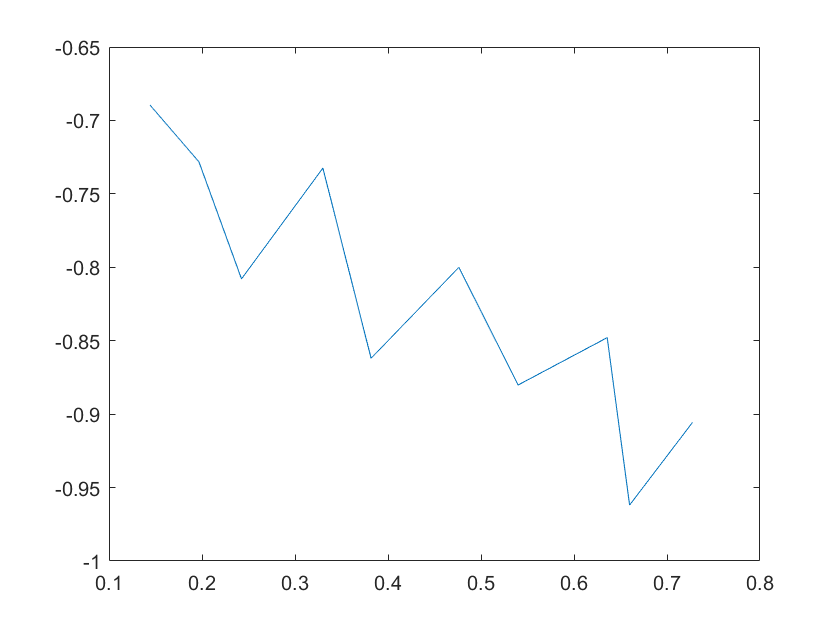
\includegraphics[height=4cm]{d8.png}
			\caption{sensitivity of kd8}
		\end{subfigure}%
		\begin{subfigure}{0.5\textwidth}
			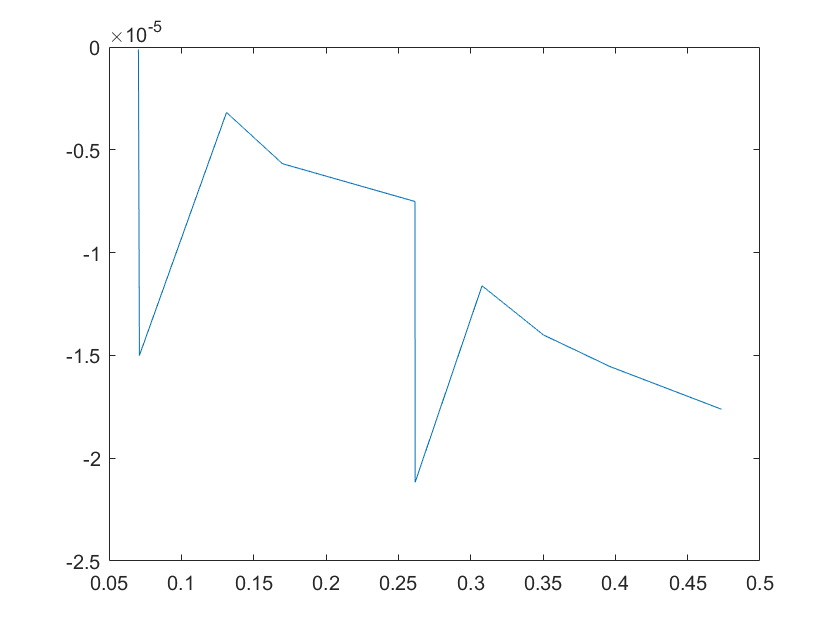
\includegraphics[height=4cm]{d9.png}
			\caption{sensitivity of kd9}
		\end{subfigure}
		\begin{subfigure}{0.5\textwidth}
			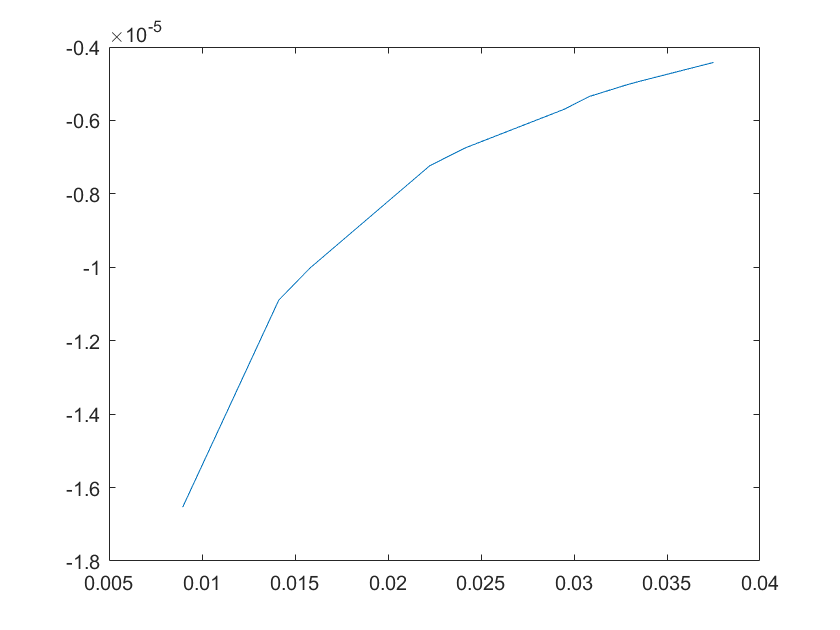
\includegraphics[height=4cm]{d10.png}
			\caption{sensitivity of kd10}
		\end{subfigure}%
		\begin{subfigure}{0.5\textwidth}
			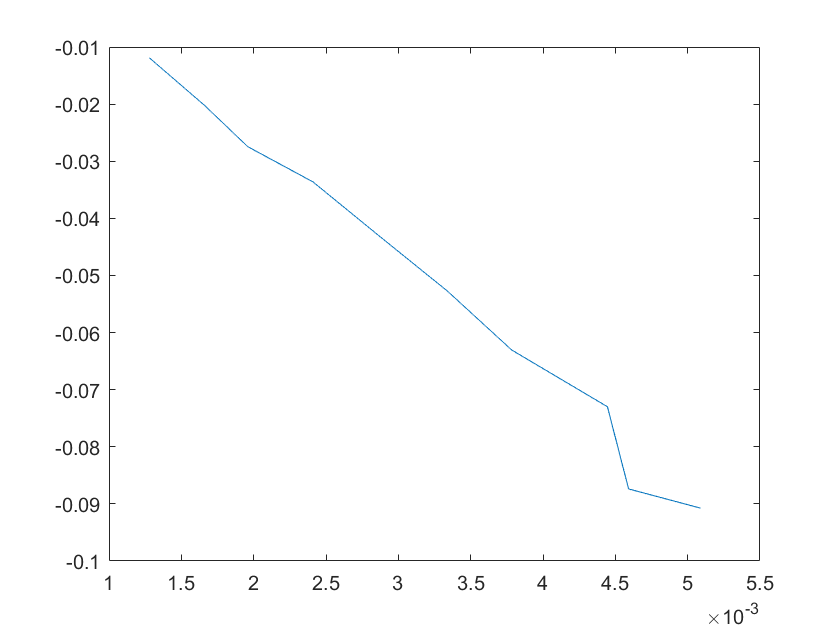
\includegraphics[height=4cm]{d11.png}
			\caption{sensitivity of kd11}
		\end{subfigure}
		\caption{Sensitivity analysis of kd6-kd11}
\end{figure}
Note:The ordinate axis represents the sensitivity S, and the abscissa axis is the parameter k for which we want to evaluate the sensitivity.
\subsection{Application of the model}
Since the goal of our project is to increase the sensitivity of biosensors by introducing a complex of dCas9-RNAP and sgRNA, and one of the purposes of our model is to explore whether this complex is effective. So we assume a reasonable and large enough concentration value for this complex. We use the concentration of glyceraldehyde-3-phosphate dehydrogenase A as the assumed concentration. Glyceraldehyde 3 phosphate dehydrogenase A (gapA) is a crucial enzyme in the glycolytic pathway, and the gene encoding this enzyme is a housekeeping gene in E. coli cells with high expression levels. We find in the literature that the protein mass of gapA is 48645fg/cell, and its molecular weight is 35492 Da.\cite{Molecular \& Cellular Proteomics} The amount of abundance of Glyceraldehyde 3 phosphate dehydrogenase A protein per cell can be calculated as follows:

\begin{displaymath}
	n=\frac{m}{M}=\frac{48645*10^{-15}g}{35492g/mol}=1.37*10^{-15}mol
\end{displaymath}

As for the size of E. coli, we found relevant data from the literature, as the figure below shows.\cite{grossman1982changes}

\begin{figure}[!htbp]
	\centering
	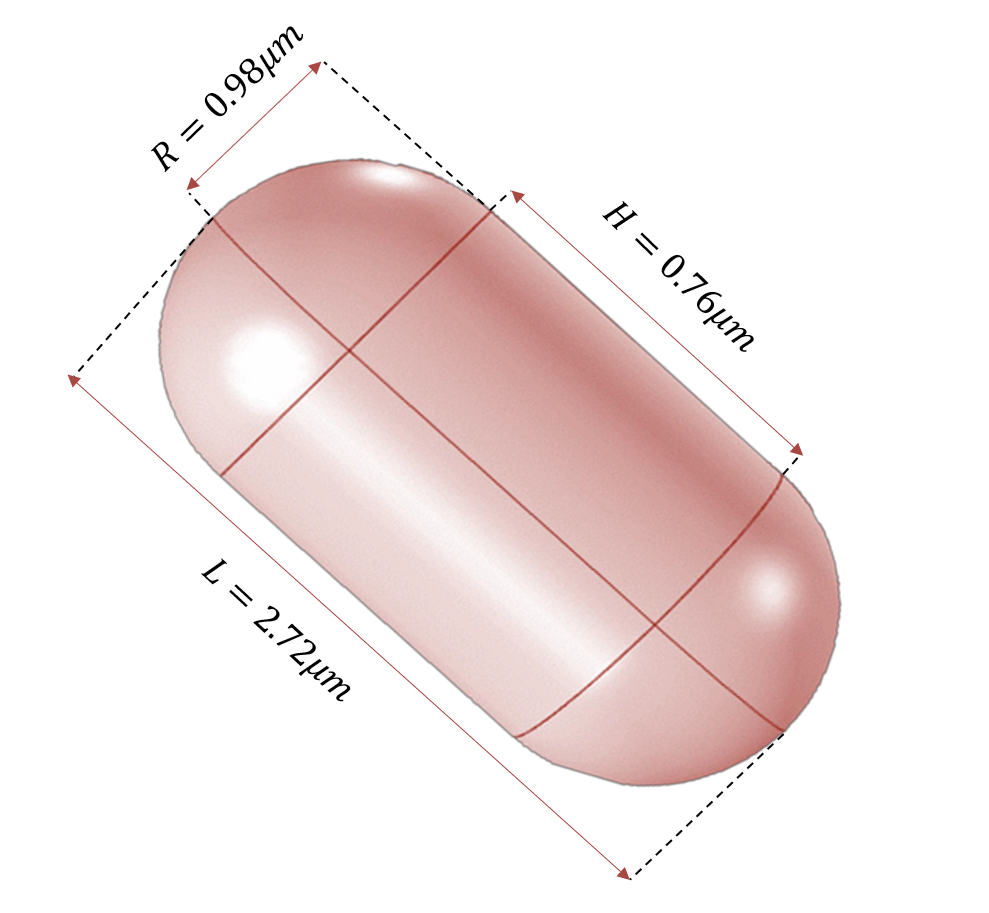
\includegraphics[width=7cm,height=7cm]{dc}
	\caption{Size of E. coli}
\end{figure}

The volume of E. coli can be calculated as follows:
\begin{displaymath}
	V_{E.coli}=\frac{4}{3} \pi R^3+\pi R^2H=\frac{4}{3} \pi (0.98\mu m)^3+\pi (0.98\mu m)^2(0.76\mu m)=6.24\mu m^3=6.24*10^{-15}L
\end{displaymath}

Then the concentration of Glyceraldehyde 3 phosphate dehydrogenase A protein in the cell can be determined:
\begin{displaymath}
	c=\frac{n}{V_{E.coli}}=\frac{1.37*10^{-15}mol}{6.24*10^{-15}L}=0.22mol/L
\end{displaymath}

With this concentration, we can get very nice results:

\begin{figure}[!htbp]
	\centering
	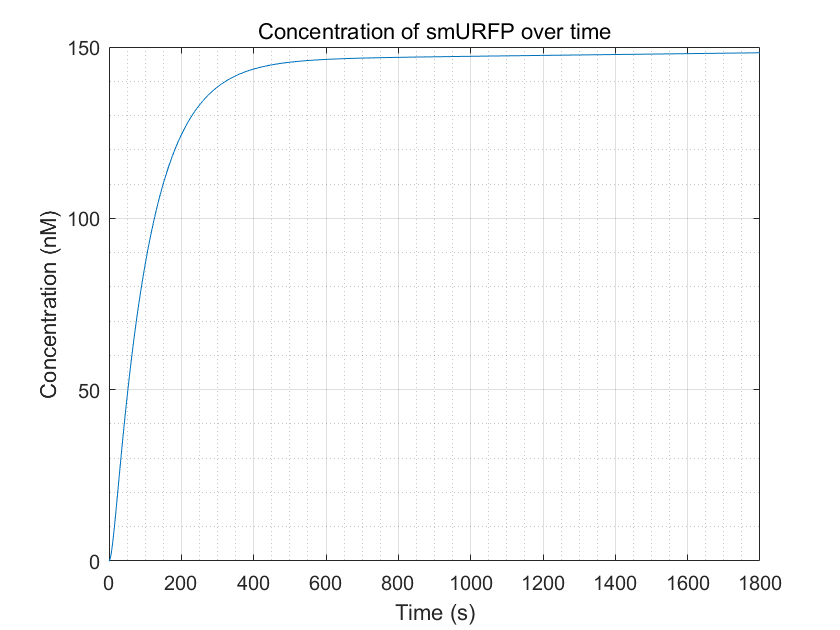
\includegraphics[width=7cm,height=7cm]{23}
	\caption{Schematic diagram of smURFP fluorescence}
\end{figure}

Compared to the diagram without introducing dCas9:

\begin{figure}[!htbp]
	\centering
	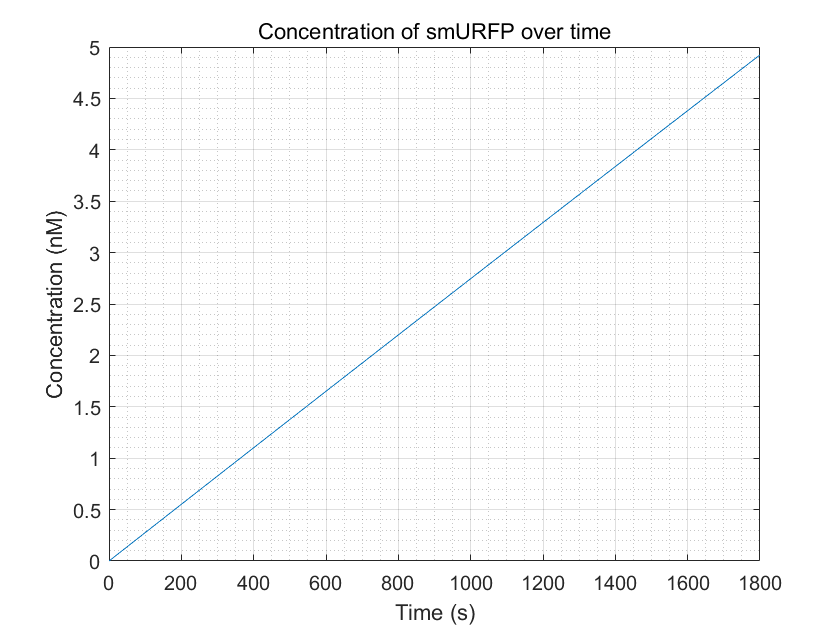
\includegraphics[width=7cm,height=7cm]{21}
	\caption{smURFP fluorescence within a reasonable time frame}
\end{figure}
\begin{figure}[!htbp]
	\centering
	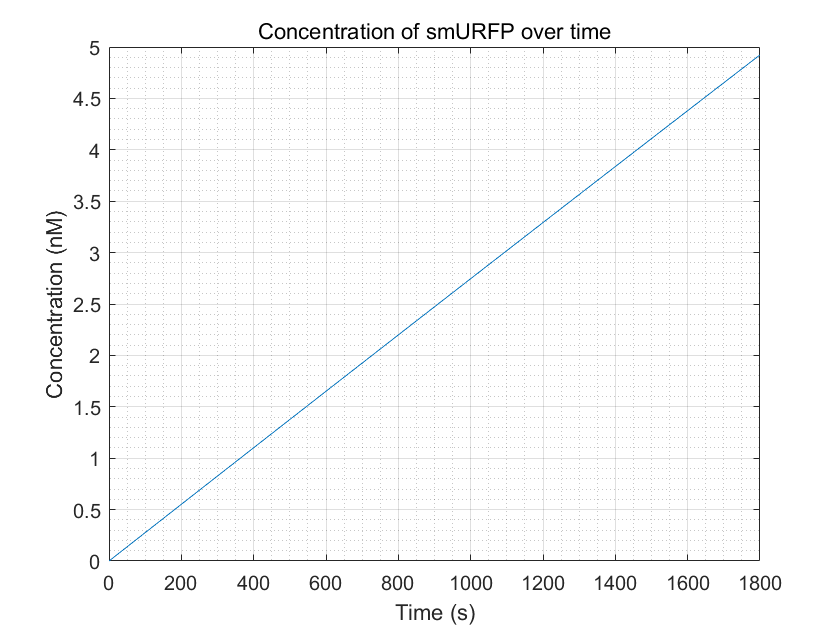
\includegraphics[width=7cm,height=7cm]{21}
	\caption{smURFP fluorescence reaches equilibrium but costs too long}
\end{figure}

From these three figures, we can conclude that dCas9-RNAP:sgRNA does have the effect of promoting transcription and increasing fluorescence intensity, thereby increasing sensitivity, as long as its concentration is sufficient. This result enhances the confidence of the experimental group, and they need to try to improve the expression of dCas9-RNAP:sgRNA in E. coli without having to doubt its role.



